\documentclass[11pt,a4paper]{article}

\usepackage[T1,T2A]{fontenc}
\usepackage[utf8]{inputenc}
%\usepackage{lmodern}
\usepackage{amsmath}
\usepackage{amsthm}
\usepackage{amssymb}
\usepackage{graphicx}
\usepackage{algorithm}
\usepackage{algorithmicx}
\usepackage{algpseudocode}
\usepackage[margin=1.1in]{geometry}
\usepackage{hyperref}

\DeclareUnicodeCharacter{00A0}{ }

\newtheorem{example}{Example}
\newtheorem{theorem}{Theorem}
\newtheorem{lemma}[theorem]{Lemma}
\newtheorem{remark}[theorem]{Remark}
\newtheorem{proposition}[theorem]{Proposition}
\newtheorem{corollary}[theorem]{Corollary}
\newtheorem{definition}[theorem]{Definition}
\newtheorem{conjecture}[theorem]{Conjecture}
\newtheorem{inequality}[theorem]{Inequality}
\newtheorem{axiom}[theorem]{Axiom}
\newtheorem{problem}[theorem]{Problem}

\renewcommand{\algorithmicrequire}{\textbf{Input:}}
\renewcommand{\algorithmicensure}{\textbf{Output:}}
\renewcommand{\baselinestretch}{1.00}

\newcommand{\abs}[1]{\mathopen| #1 \mathclose|}
\newcommand{\ddz}{\frac{d}{dz}}

\begin{document}

\title{Fast and rigorous arbitrary-precision evaluation of Legendre
polynomials and Gauss-Legendre quadrature nodes}
\author{Fredrik Johansson \and Marc Mezzarobba}
\date{}
\maketitle

\begin{abstract}
We describe an efficient strategy for rigorous
arbitrary-precision evaluation of Legendre polynomials on the unit
interval and its application in the generation of Gauss-Legendre
quadrature rules.
Our focus is on making the evaluation practical for a wide range of
realistic parameters, corresponding to the requirements of numerical
integration to an accuracy of about $100$ to $100\,000$ bits.
Our evaluation algorithm combines the summation by rectangular
splitting of several types of expansions in terms of hypergeometric
series with a fixed-point implementation of Bonnet's three-term
recurrence relation.
We then compute rigorous enclosures of the Gauss-Legendre nodes and
weights using the interval Newton method.
We provide rigorous error bounds for all steps of the algorithm.
The practicality of the approach is validated by an implementation in
the Arb library.
Our implementation achieves an order-of-magnitude speedup over
previous code for computing Gauss-Legendre nodes with simultaneous
high degree and precision, making Gauss-Legendre quadrature viable
even at very high precision.
\end{abstract}

\section{Introduction}

The Legendre polynomials $P_n(x)$ are the sequence
of orthogonal polynomials with respect to the unit weight
on the interval $(-1,1)$, normalized so that $P_n(1) = 1$.
A more concrete definition is by the generating series
\begin{equation} \label{eq:generating-series}
  \sum_{n=0}^{\infty} P_n(x) z^n
  = \frac{1}{\sqrt{1 - 2 x z + z^2}}.
\end{equation}
It is often convenient to introduce auxiliary
variables~$\theta \in [0, \pi]$ and $y \in [0, 1]$ defined by
$x = \cos \theta$ and $y = \sin \theta = \sqrt{1 - x^2}$,
where one might note that the roots of the polynomial $1 - 2 x z + z^2$ appearing
in \eqref{eq:generating-series} are $e^{\pm i \theta} = x \pm i y$.

Like other families of orthogonal polynomials, Legendre polynomials
satisfy a three-term recurrence, in this case the relation
\begin{equation} \label{eq:recurrence}
  (n + 1) P_{n+1}(x) - (2n - 1) x P_n(x) + n P_{n-1}(x) = 0,
\end{equation}
also known as Bonnet's formula, and a mixed relation
\begin{equation} \label{eq:mixed}
  (x^2 - 1) P'_n(x) = n \bigl( x P_n(x) - P_{n-1}(x) \bigl)
\end{equation}
that expresses the derivative $P_n'$ in terms of two
consecutive $P_n$.

The definition implies that $P_n$ has $n$ roots all located in $(-1,1)$.
Perhaps the most important application of Legendre polynomials
is the Gauss-Legendre quadrature rule
\begin{equation}
\int_{-1}^{1} f(x) dx \approx \sum_{i=0}^{n-1} w_i f(x_i), \qquad
w_i = \frac{2}{(1-x_i^2) [P'_n(x_i)]^2},
\label{eq:glquad}
\end{equation}
where the \emph{nodes} $x_i$ are the roots of $P_n$.
The quantity~$w_i$ is called the \emph{weight} associated
with the node~$x_i$.

For some applications in computer algebra, number theory,
mathematical physics, and experimental mathematics,
it is necessary to compute integrals to an accuracy of
hundreds of digits, and occasionally even tens of
thousands of digits~\cite{bailey2011high}.
The Gauss-Legendre formula is especially well suited for
integration of smooth functions without endpoint singularities, where it
achieves an accuracy of $p$ bits with $n = O(p)$ evaluation points.

Indeed, it is well known that~\eqref{eq:glquad} is nearly optimal among
all quadrature rules for integrands that are
well-approximated by polynomials, in particular for
analytic $f$ without singularities close to
the path of integration~\cite{kowalski1985gauss,trefethen2008gauss}.
As a special case, the $n$-point rule~\eqref{eq:glquad} is exact
when $f$ is any polynomial of degree at most $2n-1$.
In general, the error in~\eqref{eq:glquad} can be bounded in terms of
$\sup_{x \in (-1,1)} |f^{(2n)}(x)|$, or if $f$ is analytic on a domain $D$
containing $(-1,1)$, in terms of $\sup_{z \in D} |f(z)|$
and the distance from the boundary of $D$ to $(-1,1)$.
Even when the conditions are not ideal for using \eqref{eq:glquad} directly,
rapid convergence is often possible
by combining~\eqref{eq:glquad}
with adaptive subdivision of the integration path~\cite{petras2002self}.

The Gauss-Legendre scheme has the drawback
that the quadrature nodes are
somewhat inconvenient to compute.
Indeed, $P_n$ becomes highly oscillatory for
large $n$ and hence presents difficulties
for naive root-finding and polynomial evaluation methods.
The classical Golub-Welsch algorithm avoids accuracy problems
by formulating the task of computing the nodes as an eigenvalue problem~\cite{golub1969calculation},
but this approach is too slow to be practical for large~$n$.

Work by several authors in the last decade has led to asymptotic methods
that permit computing any individual node and weight for arbitrarily large $n$
in ``$O(1)$'' time, culminating in the 2014 paper by Bogaert \cite{bogaert2014iteration}.
For a review of this progress, see Townsend~\cite{townsend2015race}.
Of course, the ``$O(1)$'' bound assumes that a fixed
level of precision is used. In the prevailing literature
this generally means 53-bit IEEE 754 floating-point arithmetic.
As mentioned earlier, certain applications require
considering $p \sim n$ where~$p$ is the precision in bits,
which potentially can be in the thousands.
In addition, the available ``$O(1)$'' implementations rely in part
on heuristic error estimates without rigorously proved bounds.

The literature on arbitrary precision or rigorous evaluation
is comparatively limited.
Petras \cite{petras1999computation} gave explicit
bounds for the error $|x_k^{(i)} - x_k|$ when
the roots $x_k$ of the Legendre polynomial $P_n$
are approximated using Newton iteration
\begin{equation}
\label{eq:newton}
x^{(i+1)}_k = x^{(i)}_k - \frac{P_n(x^{(i)}_k)}{P'_n(x^{(i)}_k)}
\end{equation}
provided that the initial values $x^{(0)}_k$
are computed by a certain asymptotic formula.
However, Petras did not address the numerical evaluation of $P_n(x)$.
Fousse \cite{fousse2007accurate} discussed the rigorous implementation
of Gauss-Legendre quadrature
using generic polynomial root isolation methods together with
interval Newton iteration
for root refinement,
but did not study fast methods for large $n$.

If we assume that the precision $p$ varies,
then it is clear that any node and weight
can be computed to $p$-bit accuracy in $\widetilde{O}(n p)$ time
by performing $O(\log p)$ Newton iterations \eqref{eq:newton}
from an appropriate initial value.
As a consequence, the
full set of degree-$n$ quadrature nodes of weights
can be computed in $\widetilde{O}(n^2 p)$ time.
For numerical integration of analytic functions
where we typically have $p \sim n$, a better (indeed, optimal) estimate
than the classical $\widetilde{O}(n^3)$ bound is possible:

\begin{theorem}
\label{thm:complexity}
If $p \sim n$, then the Gauss-Legendre nodes of degree $n$ can be computed to
$p$-bit accuracy in $\widetilde{O}(n^2)$ (equivalently, $\widetilde{O}(p^2)$) bit operations.
\end{theorem}

\begin{proof}
(Sketch.)
Using the formulas in~\cite{petras1999computation},
we can compute good initial values for Newton iteration
in $\widetilde{O}(n)$ bit operations.
The Newton iteration can be performed for all roots
simultaneously using fast multipoint evaluation, which costs
$\widetilde{O}(n p)$ bit operations.
Fast multipoint evaluation is numerically unstable and
generically loses $O(n)$ bits of accuracy, but we can compensate for
this loss by using $O(n)$ guard bits
(since $p \sim n$ by assumption, this does not change the asymptotic complexity estimate)~\cite{kobel2013fast}.
\end{proof}

Completing the details
of the proof is a technical exercise.
Unfortunately, despite being elegant in theory,
the algorithm behind Theorem~\ref{thm:complexity} has high overhead
in practice. Working with expanded polynomials and
processing all roots simultaneously also results in high memory usage and
makes parallelization difficult.
We can achieve a slightly worse but still subcubic
complexity of $\widetilde{O}(n^{5/2})$
by employing
fast multipoint evaluation in a completely different way
to compute $P_n$ values in isolation,
but unfortunately that algorithm
also has high overhead~\cite{Johansson2014rectangular}.

In this work, we study fast and practical computation for variable $n$
and precision $p$ with rigorous error bounds.
Our main contribution is to give a complete evaluation strategy
for Legendre polynomials on $[-1,1]$ in ball arithmetic~\cite{vdH:ball,Johansson2017arb}.
Computing the Legendre polynomial roots, then,
is a relatively simple application of the results
in~\cite{petras1999computation} together with
the interval Newton method~\cite{moore1979methods}.

Our algorithm for evaluating Legendre polynomials switches between several methods.
In Section~\ref{sec:recurrence},
we prove practical error bounds for the standard three-term recurrence,
which can be efficiently implemented
in fixed-point arithmetic.
This method is ideal for $n$ and~$p$ up to a few hundred.
For larger $n$ or $p$, we use a fast method for evaluation
of hypergeometric series.
Section~\ref{sec:series} discusses the hypergeometric series
expansions that are preferable for different inputs and precision
(including a well-known asymptotic expansion for large $n$),
and their efficient evaluation.
In Section \ref{sec:selection}, we propose a strategy to select the
best formula for any combination of $n, p, x$.

Section~\ref{sec:bench} presents benchmark results
that compare the performance
of our algorithm
to some previous implementations
as well as the asymptotically fast algorithm in Theorem~\ref{thm:complexity}.

For computing Gauss-Legendre nodes and weights with $n \sim p$,
our algorithm has an asymptotic complexity of $\widetilde{O}(n^3)$ like
classical methods. However, our algorithm has much lower overhead,
and for parameters $p, n < 10^5$ which are most relevant to applications,
the observed running time is effectively subcubic.
Furthermore, if $p = O(1)$, the complexity reduces to $\widetilde{O}(n)$
as in the machine-precision implementations by Bogaert and others.

Our code for computing Legendre polynomials and
Gauss-Legendre nodes and weights is freely available as part of
the Arb library \cite{Johansson2017arb}.

\section{General strategy}

\label{sec:general}

We work in the framework on midpoint-radius interval arithmetic,
also called ball arithmetic.
In general, given an integer~$n$ and a ball $x = [m \pm r]$,
we want to evaluate $P_n(x)$ at~$x$,
yielding an enclosure $y = [m' \pm r']$ such that $P_n(\xi) \in y$
holds for all $\xi \in x$.

We restrict our attention to real~$x \in [-1, 1]$,
which is the most interesting part of the domain for applications.
Since $P_n(-x) = (-1)^n P_n(x)$, we can further
restrict to $0 \le x \le 1$.
Some authors suggest working with $P_n(\cos(\theta))$ instead of $P_n(x)$
directly to improve numerical stability for $x$ close to 1, but
this is not necessary in arbitrary-precision arithmetic since
a slight precision increase (of the order $O(\log n)$ bits)
works as well.

Note that, for rigorous evaluation of $P_n(z)$ with complex $z$
as well as Legendre functions of non-integer order $n$,
generic methods for the hypergeometric ${}_2F_1$ function
are applicable if $n$ is not extremely large; see~\cite{johansson2016hypergeometric}.
In addition, real $|x| > 1$ can be handled with naive numerical methods.

In view of the use of Newton's method to compute the roots,
we also need to evaluate the derivative $P'_n(x)$,
typically at the same time as $P_n(x)$ itself.
A simple option is to deduce $P'_n(x)$ from
$P_n(x)$ and $P_{n-1}(x)$ using \eqref{eq:mixed}.
When $x$ is close to $1$, though, this formula involves a
cancellation of about $\abs{\log_2(1 - x)}$ bits in the subtraction,
followed by a division by $x^2 - 1$, so that a direct evaluation
of $P'_n(x)$ may be preferable to reduce the working precision.

Our evaluation algorithms rely on ball arithmetic internally to
propagate the error bounds up to the final result.
Since some methods would produce unsatisfactorily large enclosures
when executed on input balls of radius $r > 0$, we evaluate $P_n(m)$
(with higher internal precision if necessary) and use a first-order
bound
\[ \max_{\xi \in x} |P_n(\xi) - P_n(m)|
   \le r \max_{\xi \in x} |P'_n(\xi)| \]
to separately bound the propagated error.
Similarly, we use a bound for $P''_n$ to compute a reasonably
tight enclosure for $P'_n([m \pm r])$.
Suitable bounds are given in the next lemma.

\begin{lemma} \label{lemma:prop-bound}
For $-1 \leq x \leq 1$, we have
\begin{align}
\label{eq:prop-bound}
  |P_n'(x)| &\le \min\left(\frac{n(n+1)}{2},
                          \frac{n}{\sqrt{1-x^2}}\right), \\
\label{eq:prop-bound1}
  |P_n''(x)| &\le \min\left(\frac{(n+2)(n+1)n(n-1)}{8},
                           \frac{2|x||P_n'(x)| + n(n+1)}{1-x^2}\right).
\end{align}
\end{lemma}

\begin{proof}
%$$|p^{(d)}(x)| \le \left(\frac{2n}{\sqrt{1-x^2}}\right)^d$$
%Markov: $$|p^{(d)}(x)| \le (n(n-1)\cdots(n-d+1))^2$$

Using the Bernstein inequality (see \cite{borwein2012polynomials}, chapter 5)
and the fact that $|P^{(d)}_n(x)| \le |P^{(d)}_n(1)|$ for $-1 \le x \le 1$,
we have~\eqref{eq:prop-bound}
and contiguous relations yield~\eqref{eq:prop-bound1}.
\end{proof}

Thus, from now on, we assume that $x$~is a floating-point number with
$0 \leq x \leq 1$.
Our main algorithm for evaluating~$P_n$ at~$x$ combines the following
methods:
\begin{itemize}
  \item the iterative computation of~$P_n(x)$
  via~\eqref{eq:recurrence},
  \item an asymptotic expansion of $P_n(x)$ as~$n \to \infty$,
  \item the usual terminating expansion of $P_n$ in the monomial
  basis,
  \item a similar terminating expansion at~$1$.
\end{itemize}
Up to simple prefactors, all three expansions are hypergeometric
series, i.e., sums of the form $\sum_k c_k \xi^k$ where $c_k/c_{k-1}$
is a rational function of~$k$.

The constraints and heuristics used to select between these algorithms
are described in detail below.
Roughly speaking,
the recurrence is used for small index~$n$ and precision~$p$, when~$x$
is not too close to~$1$,
the asymptotic series when $n$~is large enough, again with $x$~not too
close to~$1$,
the expansion at~$0$ for intermediate precisions and $x$~far from~$1$,
and the expansion at~$1$ when $x$ is close to~$1$.

\section{Basecase recurrence}

\label{sec:recurrence}

For small $n$, a straightforward way to compute~$P_n(x)$ is to apply
Bonnet's three-term recurrence \eqref{eq:recurrence},
starting from $P_0(x)=1$ and $P_1(x) = x$.
Computing~$P_n(x)$ by this method takes about $(M(t) + O(t))\, n$
bit operations, where $t$ is the working precision and $M(t)$ denotes the
cost of $t$-bit multiplication.
It is thus attractive for small $n$ and $t$, especially when both
$P_n(x)$ and $P'_n(x)$ are needed, since we can get $P_{n-1}(x)$ at no
additional cost.

In a direct implementation of this recurrence in ball arithmetic, the
width of the enclosures would roughly double at every iteration,
requiring to increase the internal working precision by $O(n)$ bits.
We avoid this issue by performing a pen-and-paper round-off error
analysis of the evaluation that yields a less pessimistic bound on the
accumulated error.
Additionally, the static error bound allows us to implement the
recurrence in fixed-point arithmetic, avoiding the overhead of
interval operations.

Fix $x \in [-1, 1]$, and let $p_n = P_n(x)$.
Bonnet's formula~\eqref{eq:recurrence} gives
\begin{equation} \label{eq:rec-bis}
  p_{n + 1} =
    \frac{1}{n+1}
    \bigl( (2n +1) x p_n - n p_{n-1} \bigr),
  \qquad n \geq 0.
\end{equation}
We implement this recurrence as follows.
Suppose $x = \hat x \, 2^{-t}$ with $\hat x \in \mathbb Z$.
Let $\lceil u \rfloor$ denote the integer truncation of a real
number~$u$ (any other rounding function would do).
The integer sequence $(\hat p_n)$ defined by
\begin{equation} \label{eq:rec-fxpt}
  \hat{p}_0 = 2^t, \qquad
  \hat{p}_1 = \hat x, \qquad
  \hat{p}_{n + 1} =
    \left\lceil \frac{1}{n + 1}  \bigl( (2 n + 1) \lceil \hat{x}
      \hat{p}_n 2^{- t} \rfloor - n \hat{p}_{n - 1} \bigr)
    \right\rfloor
\end{equation}
is easy to compute using only integer arithmetic, and
$\hat p_n \, 2^{-t}$ is an approximation of $p_n$.

Algorithm~\ref{alg:gmprec} provides a complete C implementation
using GMP~\cite{granlund2017}.

\begin{algorithm}[h!]
  %\algsetup{linenosize=\tiny}
  \caption{Evaluation of Legendre polynomials in fixed-point arithmetic using GMP}
  \small
  \label{alg:gmprec}
  \begin{algorithmic}[1]
    \Require An integer $x$ and $t \ge 0$ such that $|2^{-t} x| \le 1$, and $n \ge 1$
    \Ensure $p, q$ such that $|2^{-t} p - P_{n-1}(2^{-t} x)|, |2^{-t} q - P_{n}(2^{-t} x)| \le 0.75 (n+1)(n+2) 2^{-t}$
  \end{algorithmic}
\begin{verbatim}
void legendre(mpz_t p, mpz_t q, int n, const mpz_t x, int t)
{
    mpz_t tmp; int k; mpz_init(tmp);
    mpz_set_ui(p, 1);
    mpz_mul_2exp(p, p, t);
    mpz_set(q, x);
    for (k = 1; k < n; k++) {
        mpz_mul(tmp, q, x);
        mpz_tdiv_q_2exp(tmp, tmp, t);
        mpz_mul_si(p, p, -k);
        mpz_addmul_ui(p, tmp, 2*k+1);
        mpz_tdiv_q_ui(p, p, k+1);
        mpz_swap(p, q);
    }
    mpz_clear(tmp);
}
\end{verbatim}
\end{algorithm}

To bound the difference $\abs{\hat p_n \, 2^{-t} - p_n}$, we analyze
the effect on the result of a small perturbation in each iteration
of \eqref{eq:rec-bis}.
The bound is based on a classical linearity argument (compare, e.g.,
\cite{Wimp1984}) combined with generating and majorant series
techniques.

\begin{proposition} \label{prop:rec-error}
Suppose that a sequence $(\tilde p_n)_{n \geq -1}$ satisfies
$\tilde p_0 = 1$ and
\begin{equation} \label{eq:rec-pert}
  \tilde{p}_{n + 1} =
    \frac{1}{n+1}
    \bigl( (2n +1) x \tilde{p}_n - n \tilde{p}_{n-1} \bigr)
    + \varepsilon_n,
  \qquad n \geq 0.
\end{equation}
for arbitrary real numbers $\varepsilon_n$
with $\abs{\varepsilon_n} \leq \bar\varepsilon$ for all $n$.
Then we have
\[
  \abs{\tilde p_n  - P_n(x)}
  \leq \frac{(n+1)(n+2)}{4} \bar \varepsilon
\]
for all $n \geq 0$.
\end{proposition}

\begin{proof}
Let
$\delta_n = \tilde{p}_n - p_n$
and
$\eta_n = (n + 1) \varepsilon_n$.
Subtracting \eqref{eq:rec-bis} from \eqref{eq:rec-pert} gives
\begin{equation} \label{eq:rec-error}
  (n + 1) \delta_{n + 1}
  = (2 n + 1) x \delta_n - n \delta_{n - 1} + \eta_n,
\end{equation}
with $\delta_0 = 0$.
Consider the formal generating series
$\delta(z) = \sum_{n \geq 0} \delta_n z^n$
and
$\eta(z) = \sum_{n \geq 0} \eta_n z^n$.
Noting that \eqref{eq:rec-error} holds for all $n \in \mathbb{Z}$ if
the sequences $(\delta_n)$ and $(\eta_n)$ are extended by~$0$ for
$n < 0$
and using the relations
\[
  \sum_{n=-\infty}^{\infty} f_{n - 1} z^n
  = z \sum_{n=-\infty}^{\infty} f_n z^n,
  \qquad
  \sum_{n=-\infty}^{\infty} n f_{n} z^n
  = z \ddz \sum_{n=-\infty}^{\infty} f_n z^n,
\]
we see that \eqref{eq:rec-error} translates into
\[ (1 - 2 xz + z^2) z \ddz \delta (z)
   = z (x - z) \delta (z) + z \eta (z). \]
The solution of this differential equation with $\delta (0) = 0$ reads
\[ \delta(z) = p(z)  \int_0^z \eta(w) \, p(w) \, dw \]
where, cf. \eqref{eq:generating-series},
\[ p(z) = \sum_{n=0}^{\infty} p_n z^n
        = \frac{1}{\sqrt{1 - 2 xz + z^2}}. \]
This is an exact expression of the ``global'' error $\delta$ in terms
of the ``local'' errors~$\varepsilon_n$.

Denote by $[z^n] f(z)$ the coefficient of index $n$ in a power
series $f(z)$.
If $f$, $g$, $\hat f$, $\hat g$ are power series such that
$\abs{[z^n] f} \leq [z^n] \hat f$ and
$\abs{[z^n] g} \leq [z^n] \hat g$
for all $n$, then also
$\abs{[z^n] \int_0^z f} \leq [z^n] \int_0^z \hat f$ and
$\abs{[z^n] (fg)} \leq [z^n] (\hat f \hat g)$.
Since $\abs{p_n} = \abs{P_n(x)} \leq 1$
and $\abs{\eta_n} \leq (n+1) \bar \varepsilon$,
it follows that
\[
  \abs{\delta_n}
  = \left| [z^n] \left( p(z)  \int_0^z \eta(w) \, p(w) \, dw \right) \right|
  \leq [z^n] \left(
    \frac{1}{1-z}
    \int_0^z \frac{\bar \varepsilon}{(1 - w)^2} \frac{1}{1-w} dw \right)
\]
and therefore
\[
  \abs{\delta_n}
  \leq [z^n] \left( \frac12 \frac{\bar \varepsilon}{(1-z)^3} \right)
  = \frac{(n+1)(n+2)}{4} \, \bar \varepsilon. \qedhere
\]
\end{proof}

\begin{corollary}
Suppose that $x = \hat x \, 2^{-t}$ for some $t \geq 0$ and
$\hat x \in \mathbb Z$.
The sequence $(p_n)_{n \geq 0}$ defined by \eqref{eq:rec-fxpt}
satisfies
\[
  \abs{ \hat p_n 2^{-t} - p_n }
  \leq 0.75 \, (n+1) (n+1) \, 2^{-t},
  \qquad
  n \geq 0.
\]
\end{corollary}

\begin{proof}
We can write
\[
  \hat{p}_{n + 1} = \frac{1}{n + 1}  \bigl((2 n + 1)  (\hat{x} \,
        \hat{p}_n \, 2^{- t} + \alpha_n) - n \, \hat{p}_{n - 1}\bigr)
        + \beta_n
\]
for some $\alpha_n$, $\beta_n$ of absolute value at most one, and
hence
\[
  \hat{p}_{n + 1} = \frac{1}{n + 1}  \bigl((2 n + 1) \, \hat{x} \,
  \hat{p}_n \, 2^{- t} - n \, \hat{p}_{n - 1}\bigr) + \varepsilon_n,
  \qquad
  \varepsilon_n = \frac{2 n + 1}{n + 1} \alpha_n + \beta_n.
\]
where $\abs{\varepsilon_n} \leq 3$.
Proposition \ref{prop:rec-error} applied to
$\tilde p_n = \hat p_n \, 2^{-t}$
then provides the desired bound.
\end{proof}

We currently do not use fast evaluation techniques for large~$n$ in
combination with this recurrence, since the series expansions to be
presented next work very well in this case.

\section{Series expansions}

\label{sec:series}

For moderately large $n$, we use series expansions of $P_n(x)$ with
respect to either $n$ or $x$ rather than the algorithm from the
previous section.
The coefficients of the series are also computed by recurrence,
but fewer than $n$ terms will typically be required.
Additionally, the expansions are of a form suitable for fast
evaluation by rectangular splitting.
Let us first review the various series expansions that we are using
(an asymptotic expansion as $n \to \infty$, series expansions at $x=0$
and $x=1$), and then discuss their efficient evaluation.

\subsection{Asymptotic series}

For fixed $|x| < 1$ or equivalently $x = \cos(\theta)$ with $0 < \theta < \pi$,
an asymptotic expansion for $P_n(x)$ as $n \to \infty$
can be given as (\cite{Bogaert2012}, (3.4))
\begin{equation}
\label{eq:asymptotic}
P_n(\cos(\theta)) = \left(\frac{2}{\pi \sin(\theta)}\right)^{1/2}
\sum_{k=0}^{K-1} C_{n,k} \frac{\cos(\alpha_{n,k}(\theta))}{\sin^k(\theta)}
+ \xi_{n,K}(\theta)
\end{equation}
where
\begin{equation}
C_{n,k} = \frac{[\Gamma(k+1/2)]^2 \Gamma(n+1)}{\pi 2^k \Gamma(n+k+3/2) \Gamma(k+1)},
\end{equation}
\begin{equation}
\alpha_{n,k}(\theta) = (n+k+1/2) \theta - (k+1/2) \pi / 2,
\end{equation}
and the error term satisfies
\begin{equation}
\label{eq:truncerr0}
|\xi_{n,K}(\theta)| < 2 \left(\frac{2}{\pi \sin(\theta)}\right)^{1/2} \frac{C_{n,K}}{\sin^K(\theta)}.
\end{equation}

The coefficients $C_{n,k}$ are a hypergeometric sequence with
$$\frac{C_{n,k}}{C_{n,k-1}} = \frac{(2k-1)^2}{k (2n+2k+1)}, \quad C_{n,0} = \frac{1}{\sqrt{\pi}} \frac{4^n}{(n+\tfrac{1}{2}) {2n \choose n}}.$$

To evaluate the error bound, we can use the following inequality for $n, k \ge 1$:
\begin{equation}
\label{eq:truncerr0b}
C_{n,k} \le \frac{1}{\pi n^{1/2}} \frac{k! n!}{2^k (n+k)!} \le \frac{1}{\pi n^{1/2}} \frac{k!}{(2n)^k}.
\end{equation}

The asymptotic expansion is in fact a convergent series
when $2 \sin(\theta) > 1$, which allows evaluating $P_n(x)$ to unbounded
accuracy for fixed $n$ when $\tfrac{1}{6}\pi < \theta < \tfrac{5}{6} \pi$.
The particular form \eqref{eq:asymptotic}
must be used for this purpose; there is a slightly different version of the expansion
which is asymptotic to $P_n(x)$ (for fixed $K$ when $n \to \infty$)
but paradoxically
converges to $2 P_n(x)$ (for fixed $n$ when $K \to \infty$); see \cite{Olver1997} and \cite{Olver2010}.

We can restate \eqref{eq:asymptotic} as a hypergeometric series
by working with complex numbers.
Letting $\omega = 1 - (x/y) i$, with $x = \cos(\theta)$ and $y =
\sin(\theta)$ as usual, we have
\begin{equation}
\label{eq:asymptoticcomplex}
P_n(x) = \sqrt{\pi y} \, \operatorname{Re}\left[
(1-i) (x+y i)^{n+1/2}
\sum_{k=0}^{K-1} C_{n,k} \omega^k\right] + \xi_{n,K}(\theta).
\end{equation}
This eliminates the explicit trigonometric functions and permits using
Algorithm~\ref{alg:hyprs} below to evaluate the series.

\subsection{Expansion at zero}

If $n = 2d$ is even, the expansion of $P_n(x)$ on the monomial basis
reads
$$P_{2d}(x) = (-1)^d \sum_{k=0}^d \frac{(-1)^k}{2^n} {n \choose d-k} {n+2k \choose n} x^{2k} = \frac{(-1)^d}{2^{2d}} {2d \choose d} \sum_{k=0}^d A_{-1}(d,k) (-x^2)^k,$$
and if $n = 2d+1$ is odd, we have
\begin{align*}
P_{2d+1}(x) &= (-1)^d x \sum_{k=0}^d \frac{(-1)^k}{2^n} {n \choose d-k} {n+2k+1 \choose n} x^{2k} \\
&= \frac{(-1)^d (d+1)}{2^{2d+1}} {2d+2 \choose d+1} \,x\, \sum_{k=0}^d A_{+1}(d,k) (-x^2)^k
\end{align*}
where $A_{\pm 1}(d,0) = 1$ and
$$\frac{A_{\sigma}(d,k)}{A_{\sigma}(d,k-1)} = \frac{(d-k+1) (2d+2k+\sigma)}{k (2k+\sigma)}.$$

If the series are truncated after the $k = K - 1$ term
(for any $K < d + 1$), the error is bounded by the first
omitted term times $(1-\alpha)^{-1}$
where
\begin{equation}
\label{eq:truncerr1}
\alpha = |x|^2 \frac{(d-K+1)(2d+2K+\sigma)}{K (2K+\sigma)}.
\end{equation}

The expansion at zero involves no cancellation
when applied to an imaginary argument.
Solving the majorizing recurrence $f_n = 2 |z| f_{n-1} + f_{n-2}$ with
$f_0 = 1$, $f_1 = |z|$ shows that
\[ |P_n(z)| \le |P_n(i|z|)| \le \left(|z| + \sqrt{1 + |z|^2}\right)^n. \]
Therefore, the possible cancellation assuming that $|P_n(x)| \approx 1$
is about $n \log_2(|x| + \sqrt{1 + |x|^2})$ bits
(which is at most $(\log_2 (1+\sqrt{2})) n \approx 1.27156n$).

\subsection{Expansion at one}

Expanding at $x = 1$ yields
$$P_n(x) = \sum_{k=0}^n c_{n,k} u^k, \quad c_{n,k} = {n \choose k} {n+k \choose k}$$
where $u = (x-1)/2$.
The coefficients $c_{n,k}$ are hypergeometric with
ratio $c_{n,k}/c_{n,k-1} = (n-k+1)(n+k)/k^2$
and initial value $c_{n,0} = 1$.

If the series is truncated after the $k = K - 1$ term,
the error is bounded by
\begin{equation}
\label{eq:truncerr2}
{n \choose K}{n+K \choose K} |u|^K \frac{1}{1-\alpha}, \quad \alpha = |u| \frac{(n-K)(n+K+1)}{(K+1)^2}.
\end{equation}

For $u \ge 0$, the series does not suffer from cancellation.
For $u < 0$, we can estimate the amount of
cancellation from the magnitude of $P_n(x')$ where $|u| = (x'-1)/2$.
For not too large $x' \ge 1$, a very good approximation is
$$P_n(x') \approx \sum_{k=0}^{\infty} \frac{n^{2k}}{(k!)^2} u^k = I_0(2n\sqrt{u}) \approx e^{2n\sqrt{u}}.$$
We therefore need about $2n\sqrt{\max(0,-u)} / \log(2)$ bits
of increased precision when evaluating the series.

We can compute $P'_n$ from $P_n$ and $P_{n-1}$, but since this
involves a division by $1-x^2$, it is useful to evaluate
evaluate $P'_n$ directly when $x$ is close to 1.
We have
$P'_n(x) = \sum_{k=0}^{n-1} c'_{n,k} u^k$
where $c'_{n,k} = (k+1) c_{n,k+1} / 2$ satisfies
\[
  c'_{n,0} = \frac{n(n+1)}{2}, \qquad
  \frac{c'_{n,k}}{c'_{n,k-1}} = \frac{(n-k)(n+k+1)}{k(k+1)}.
\]
Since $c'_{n,k} \le n c_{n,k+1}$, the truncation error is bounded by
\begin{equation}
\label{eq:truncerr2b}
n {n \choose K+1}{n+K+1 \choose K+1} |u|^K \frac{1}{1-\alpha}
\end{equation}
with $u$ and $\alpha$ as above.

\subsection{Hypergeometric series evaluation}

\label{sec:serieseval}

We use rectangular splitting~\cite{Smith1989,Johansson2014rectangular}
for fast evaluation of hypergeometric series with
rational parameters where the argument $x$ is a high-precision number.
This reduces evaluating a $K$-term series to
$O(K)$ cheap scalar operations (additions and multiplications or divisions
by small integer coefficients)
and about $2\sqrt{K}$ expensive nonscalar operations (general multiplications),
whereas direct evaluation of the hypergeometric
recurrence requires $O(K)$ expensive operations.

Due to the scalar operations, rectangular splitting ultimately
requires $O(K)$ arithmetic operations with $\widetilde{O}(p)$ bit complexity
each
just like straightforward evaluation of the recurrence, so it is
not a genuine asymptotic improvement, but in practice this
algorithm is still faster even at moderate precision
and can give more than a factor 100 speedup at very high precision.
It is possible to genuinely reduce the complexity of evaluating
a hypergeometric sequence to $O(\sqrt{K} \log(K))$ arithmetic
operations using a baby-step giant-step method
that employs fast multipoint evaluation,
but in practice rectangular splitting
performs better until both $K$ and the bit precision
exceed $10^6$ (see \cite{Johansson2014rectangular}).

Another technique for fast evaluation of hypergeometric series,
binary splitting, would be useful when $p$ is large and the
argument $x$ is a rational number with small numerator and denominator,
but this case is not relevant for our application.

\begin{algorithm}[h!]
  %\algsetup{linenosize=\tiny}
  \caption{Evaluation of hypergeometric series using rectangular splitting}
  \small
  \label{alg:hyprs}
  \begin{algorithmic}[1]
    \Require An arbitrary $x$, recurrence data $p, q \in \mathbb{Z}[k]$, integer $K \ge 0$, offset $\Omega \in \{0,1\}$.
    \Ensure $s = \sum_{k=\Omega}^{K-1} x^k \prod_{j=\Omega}^k p(j) / q(j)$
    \State $m \gets \lfloor \sqrt K \rfloor$; precompute $[1, x, x^2, \ldots, x^m]$ \Comment{Tuning parameter: any $m \ge 1$ can be used}
    \State $s \gets 0; \quad k \gets K - 1$
    \While{$k \ge \Omega$}
        \State $u \gets \min(4, k + 1 - \Omega)$  \Comment{Tuning parameter: any $1 \le u \le k+1-\Omega$ can be used}
        \State $(a, b) \gets (k - u + 1, k)$  \Comment{Unrolled range}
        \State $c \gets \prod_{j=a}^b p(j)$ \Comment{Small integer coefficient}
        \While{$k \ge a$}
            \State $r \gets k \bmod m$
            \If{$k = b$}
                \State $s \gets c \cdot (s + x^r)$ \Comment{Using precomputed power of $x$}
            \Else
                \State $s \gets s + c \cdot x^r$ \Comment{Using precomputed power of $x$}
            \EndIf
            \If{$r = 0$ \textbf{and} $k \ne 0$}
                \State $s \gets s \cdot x^m$ \Comment{Using precomputed power of $x$}
            \EndIf
            \State $c \gets (c / p(k)) q(k)$ \Comment{Exact small integer division}
            \State $k \gets k - 1$
        \EndWhile
        \State $s \gets s / c$
    \EndWhile
    \State \Return $s$
  \end{algorithmic}
\end{algorithm}

Algorithm \ref{alg:hyprs} presents our version of rectangular splitting
for the present application.
This algorithm is a generalization of the
method for evaluating Taylor series of elementary
functions given in~\cite{Johansson2015elementary},
which combines rectangular splitting
with partially unrolling the recurrence to reduce the number of scalar divisions
(which in practice are more costly than scalar multiplications).
The terms are computed in the reverse direction to allow
using Horner's rule for the outer
multiplications.

Our implementation uses ball arithmetic for $x$ and $s$
so that no error analysis is needed, and we use a bignum type for $c$ (so
no overflow can occur regardless of $u$);
for low precision a faster implementation
would be possible using fixed-point arithmetic with tight
control of the word-level operations
as was done for elementary functions in~\cite{Johansson2015elementary}.

The algorithm contains two tuning parameters.
The splitting parameter $m$ controls the
number $m$ of multiplications for powers versus the number $K / m$ of
multiplications for Horner's rule.
The choice $m \approx \sqrt K$ is optimal,
but when evaluating two series for the same~$x$
(in our case, to compute both $P_n(x)$ and $P'_n(x)$),
the table of powers can be reused,
and then $m \approx \sqrt{2K}$ minimizes the total cost.

The unrolling parameter $u$ controls the number of coefficients
to collect on a single denominator, reducing the
number of divisions to $N / u$.
Ideally, $u$ should be chosen
so that $\prod_{j=a}^b p(j)$
and $\prod_{j=a}^b q(j)$ fit in 1 or 2 machine words.
The example value $u = 4$ is a reasonable
default, but as an optimization, one might vary $u$
for each iteration of the main loop
to ensure that $c$ always fits in a specific number of words.

The redundant parameter $\Omega$ is a small convenience in the pseudocode.
Setting $\Omega = 1$ and adding the constant term separately
avoids having to make a special case to prevent division by zero
when $q(0) = 0$.

\subsection{Binomial coefficients}

The prefactors of both the series expansion at $x = 0$ and the asymptotic series
contain the central binomial coefficient ${2n \choose n}$.
We need to compute this factor efficiently for any $n$ and precision $p$.
Since ${2n \choose n} \approx 4^n$, it is best to use
an exact algorithm when $n < Cp$ for some small constant $C > 1/2$.
We use the binomial function provided by GMP for $n < 6p + 200$
and otherwise use an asymptotic series for ${2n \choose n}$
with error bounds given in~\cite{brent2016asymptotic}.

We also need to quickly estimate the magnitude of binomial coefficients
for error bounds of series truncations.
We have the binary entropy estimate
$$\log_2 {n \choose k} \le n G(k/n), \quad G(x) = -x \log_2(x) - (1-x) \log_2(1-x)$$
and the equivalent form
\begin{equation}
\label{eq:binbound}
{n \choose k} \le \left(\frac{n}{n-k}\right)^{n-k} \left(\frac{n}{k}\right)^k = \frac{n^n}{k^k (n-k)^{n-k}}.
\end{equation}
The function $G(x)$ can be evaluated cheaply with a precomputed
lookup table (only a coarse estimate is needed).

\section{Algorithm selection}

\label{sec:selection}

We first use a set of simple heuristic cutoffs found experimentally to decide whether to use the basecase recurrence or one of the series expansions. The recurrence is mainly faster for some combinations of $p < 1000$, $n < 400$ when computing $(P_n(x), P'_n(x))$ simultaneously and for some combinations of $p < 500$, $n < 100$ when computing $P_n(x)$ alone (in all cases subject to some boundaries $\varepsilon < x < 1 - \varepsilon$); the actual optimal regions are complicated due to differences in overhead between fixed-point integer arithmetic and ball arithmetic for the respective algorithm implementations. For the actual cutoffs used, we refer to the source code.

To select between the series expansion at $x = 0$, the expansion at $x = 1$, and the asymptotic series, the following heuristic is used. For each algorithm $A$, we estimate the evaluation cost as $C_A = K_A (p + p_A)$ where $K_A$ is the number of terms required by algorithm~$A$ ($K_A = \infty$ if $A$ is the asymptotic series and it does not converge to the required accuracy), $p$ is the precision goal, and $p_A$ is the extra precision required by algorithm $A$ due to internal cancellation. For the asymptotic series, we multiply the cost by an extra factor 2 as a penalty for using complex numbers. In the end, we select the algorithm with the lowest $C_A$.

We select $K_A$ and estimate $p_A$ heuristically using machine precision
floating-point computations, working with logarithmic magnitudes to
avoid underflow and overflow.
During the actual evaluation of the series expansions, $K_A$ and $p_A$ are then given;
we compute rigorous upper bounds
for the truncation error via
\eqref{eq:truncerr0}, \eqref{eq:truncerr0b}, \eqref{eq:truncerr1},
\eqref{eq:truncerr2}, \eqref{eq:truncerr2b}, \eqref{eq:binbound}
using floating-point arithmetic with directed rounding,
while additional rounding errors are tracked by the ball arithmetic.

\begin{figure}[h!]
\begin{centering}
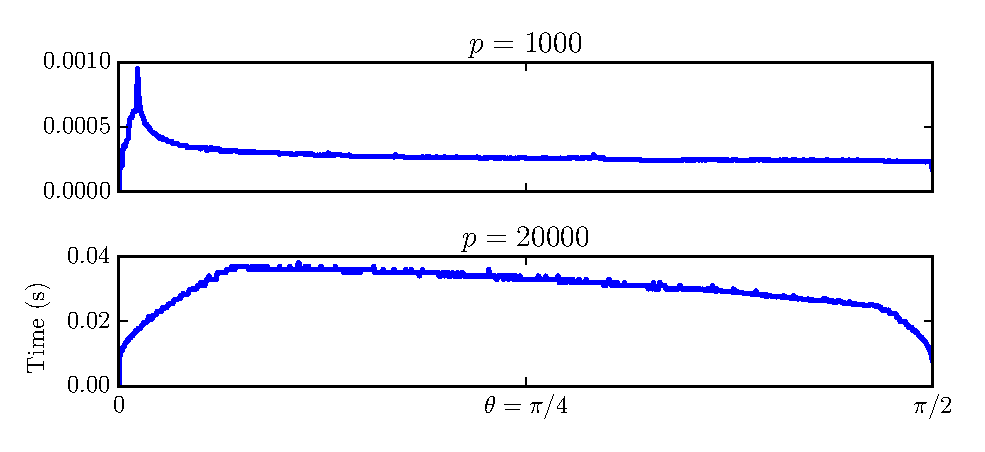
\includegraphics[width=0.8\textwidth]{timeplot}
\caption{Time to evaluate $(P_n(x), P'_n(x))$ at the location of the root $x = r_{n,k}$ for $0 \le k < n/2$, at varying levels of precision $p$.
The separate timing curves in each plot are for $p = 64, 256, 1024, 4096, 16384$, and each curve has been normalized by setting its median height to 1. The $y$ axis for the $n = 10^5$ timings has been cut off; the highest peak is $y \approx 24$ times the median which occurs at $k = 6$ when $n = 10^5$ and $p = 64$.}
\label{fig:timeplot}
\end{centering}
\end{figure}

The assumption that the running time is a bilinear function of $K_A$ and $p + p_A$ is not completely realistic, but this cost estimate nonetheless captures the correct asymptotics when
$$x \to 0, \quad x \to 1, \quad n \to \infty, \quad p \to \infty$$
separately, and hopefully will not be too inaccurate in the transition regions. This is verified empirically. The plots in Figure~\ref{fig:timeplot} show the measured timings to evaluate $(P_n(x), P'_n(x))$ at $x = r_{n,k}$ where $r_{n,k}$ is the root with index $k$ (where $k/n = 0$ is closest to $x = 1$ and $k/n = 1/2$ is closest to $x = 0$), using the automatic algorithm selection. The individual curves show the time at respective precisions $p = 64, 256, 1024, 4096, 16384$. Each curve has been normalized by its median height, i.e.\ the median time to compute any root with a fixed $(n,p)$ is set to 1.

For large $n$ and $p \ll n$, a sharp peak appears at the transition between the series expansion at $x = 1$ and the asymptotic expansion. This peak could presumably be removed by use of an asymptotic method for large $n$ valid when $x \approx 1$. However, the extra area under the peak compared to the area under the median baseline is so small that generating the full set of Gauss quadrature nodes would not be sped up much.

\section{Benchmarks}

\label{sec:bench}

\subsection{Polynomial evaluation}

\begin{figure}[h!]
\begin{centering}
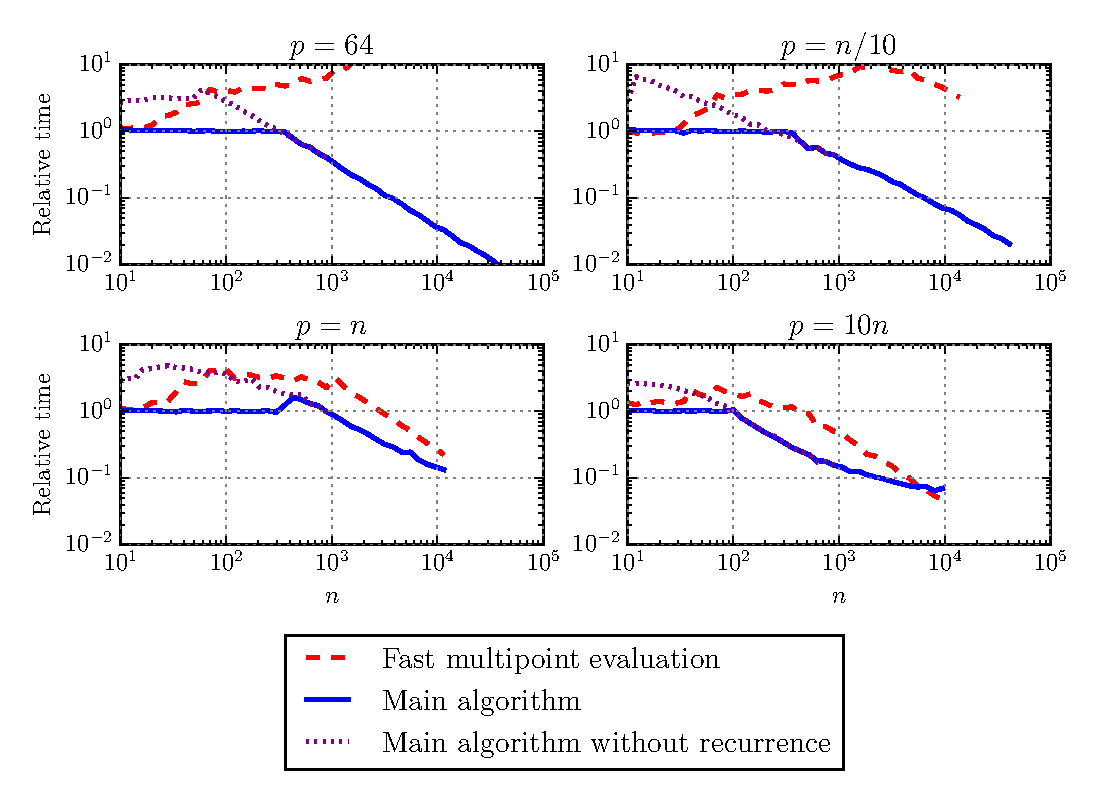
\includegraphics[width=0.8\textwidth]{benchplot}
\caption{Performance comparison of various methods to evaluate $(P_n(x), P'_n(x))$ to $p$-bit precision for a
set of $n / 2$ points $0 < x < 1$ distributed like the roots of $P_n$.
The $y$ axis (relative time) shows the time divided by the time
using the three-term recurrence in fixed-point arithmetic.}
\label{fig:benchplot}
\end{centering}
\end{figure}

Figure~\ref{fig:benchplot} compares the performance of different methods
for evaluating $(P_n(x), P'_n(x))$ on a set of $n/2$ points
distributed like the positive roots of $P_n(x)$
to simulate one stage of Newton iteration at $p$-bit precision.
The following four methods are timed:

\begin{itemize}
\item The time for evaluation using the three-term recurrence is set to 1, i.e.\ we divide
the other timings by this measurement.
\item The solid curves show the time using our hybrid method
(from here on called the ``main algorithm'')
with automatic selection between the three-term
recurrence and different
series expansions.
\item The dotted curves show the time using the main algorithm without
the three-term recurrence as the basecase, i.e.\ using series expansions
even for very small $n$.
\item The dashed curves show the time for fast multipoint
evaluation of the expanded polynomials $P_n(x)$ and $P'_n(x)$.
Technically, we expand
$P_{n}(\sqrt{x})$ for even $n$ and $P_{n}(\sqrt{x})/\sqrt{x}$ for odd $n$
and evaluate at $x^2$ since this halves the amount of work.
The polynomial coefficients are generated in advance using
the hypergeometric recurrence and
the fast multipoint evaluation is done using
the Arb function \texttt{\_arb\_poly\_evaluate\_vec\_fast\_precomp}
(where the ``precomp'' suffix indicates that
the same product tree is used for both $P_n$ and $P'_n$).
The fast multipoint evaluation is done with $2.9n$ guard bits,
which was found experimentally to be sufficient for full accuracy.
\end{itemize}

The crossover point between the
three-term recurrence and series expansions usually occurs
around $n \approx 10^2 - 10^3$ (it can be as low as $n \approx 10$
if $p$ is much larger).
For modest $n$,
the three-term recurrence is much faster
than the hypergeometric series (typically by a factor 3-4)
due to working with negligible extra precision
and due to the low-overhead fixed-point arithmetic.
This low overhead is very useful for typical evaluation of
Legendre polynomials and generation of quadrature nodes
for one or a few machine words of precision.
The crossover point could be lowered slightly
if we used a similarly optimized fixed-point implementation
for the hypergeometric series.

When $p$ is fixed (top left in Figure~\ref{fig:benchplot}), the main algorithm is
a factor $O(n)$ faster
than the three-term recurrence
since the asymptotic expansion converges to sufficient accuracy after
$O(1)$ terms for all sufficiently large $n$.
With the constant precision $p = 64$,
the main algorithm is 3.0
times faster for $n = 10^3$ and 30 times faster for $n = 10^4$.
Conversely, fast multipoint evaluation
with constant $p$ is a factor $O(n)$ slower due to the $O(n)$ extra precision.

When $p \sim n$ (the three remaining plots in Figure~\ref{fig:benchplot}), the main algorithm
appears to show the same $O(n)$ speedup
over the three-term recurrence after the crossover point, at least initially.
This speedup should level off asymptotically, but
in practice this only occurs for $n$ larger than $10^4$
where we have already gained a factor 10 or more.

Fast multipoint evaluation gives a true asymptotic $O(n)$ speedup,
but since it has much higher overhead,
it only starts to give an improvement over
the main algorithm from $n \approx 10^4$
and for $p$ larger than $n$.
When $p = n / 10$, it appears that
fast multipoint evaluation will only break even for $n$ much larger than $10^5$.
We conclude that fast multipoint evaluation would be
worthwhile only for the last few Newton iterations
when computing quadrature nodes for exceptionally high precision.
Since independent evaluations are more convenient and easy to parallelize,
the fast multipoint evaluation method
currently seems to have limited practical value for this application.

\subsection{Quadrature nodes}

The Arb function \texttt{arb\_hypgeom\_legendre\_p\_ui\_root(x, w, n, k, p)}
sets the output variable
$x$ to a ball containing the root of $P_n$ with index $k$ (we use the indexing
$0 \le k < n$, with $k = 0$ giving the root closest to 1),
computed to $p$-bit precision.
It also sets $w$ to the corresponding quadrature weight.
We use the formulas in \cite{petras1999computation} to
compute an initial enclosure with roughly machine precision,
followed by refinements with the interval Newton method
at doubling precision steps for very high precision.

\begin{table}[h!]
\begin{centering}
\begin{tabular}{ c | c c c c c }
$n\, \backslash \; p$ & 64 & 256 & 1024 & 3333 & 33333 \\ \hline
20  & 0.000149  &  0.000300  &  0.000660  &  0.00149  &  0.0217  \\ 
50  & 0.000540  &  0.00119  &  0.00267  &  0.00590  &  0.0760  \\ 
100  & 0.00181  &  0.00380  &  0.00900  &  0.0188  &  0.205  \\ 
200  & 0.00660  &  0.0141  &  0.0310  &  0.0640  &  0.624  \\ 
500  & 0.0289  &  0.0850  &  0.214  &  0.384  &  2.80  \\ 
1000  & 0.0660  &  0.174  &  0.625  &  1.36  &  9.68  \\ 
2000  & 0.106  &  0.362  &  1.20  &  4.52  &  34.3  \\ 
5000  & 0.235  &  0.815  &  2.92  &  14.6  &  189  \\ 
10000  & 0.480  &  1.63  &  5.49  &  27.3  &  694  \\ 
100000  & 4.90  &  16.1  &  49.6  &  221  &  13755  \\ 
1000000  & 73.0  &  195  &  512  &  2016  &  105705
\end{tabular}
\caption{Time in seconds to compute the set of degree-$n$ Gauss-Legendre nodes and weights with $p$-bit precision.
(For large $n$ and $p$, the time was estimated by computing a subset of the nodes and weights.)}
\label{tab:timings}
\end{centering}
\end{table}

Table~\ref{tab:timings} shows absolute timings for computing
degree-$n$ Gauss-Legendre nodes to $p$-bit precision
by calling this function repeatedly with $0 \le k < n / 2$.
The timings were obtained on a 1.90 GHz Intel Core i5-4300U CPU
using a single core.

For low precision and large $n$, our implementation
is about three orders of magnitude slower than the machine precision
code by Bogaert \cite{bogaert2014iteration}
which is reported to compute the nodes and weights for $n = 10^6$
in 0.02 seconds on four cores.
This difference is reasonable since we use arbitrary-precision arithmetic,
compute rigorous error bounds, and evaluate the Legendre polynomials
explicitly whereas Bogaert uses a more sophisticated
asymptotic development for both the nodes and the weights.

We also note that we can compute 53-bit floating-point values
with provably correct rounding in about the same time as the 64-bit
values (for a ball with relative radius just larger than $2^{-64}$, there
is less than a $1\%$ probability that the correct 53-bit rounding
cannot be determined, in which case that particular node
can be recomputed with a few more bits).

Fousse~\cite{fousse2007accurate} reports a few timings for smaller $n$ and high precision
obtained on a 2.40 GHz AMD Opteron 250 CPU.
For example, $n = 80, p = 500$ takes 0.14 seconds (our implementation
takes 0.037 seconds) and $n = 556, p = 5000$ takes 17 seconds
(our implementation takes 0.61 seconds).

The \texttt{mathinit} program included with version 2.2.19
of D.\ H.\ Bailey's ARPREC library
generates Gauss-Legendre quadrature nodes
using Newton iteration together with the three-term recurrence for evaluating
Legendre polynomials~\cite{bailey2002arprec,bailey2011high}.
With default parameters, this program computes the rules of degree $n = 3 \cdot 2^{i+1}$
for $1 \le i \le 10$ at 3408 bits of precision, intended as
a precomputation for performing
degree-adaptive numerical integrations with up to 1000 decimal digit accuracy.
This takes about 1300 seconds (our implementation takes 33 seconds).
A breakdown for each degree level
is shown in Table~\ref{tab:arprectimings}.

\begin{table}[h!]
\begin{centering}
\begin{tabular}{ c | c c | c c| c c | c c }
$n$ & ARPREC & Our code &
    \multicolumn{2}{|c|}{$\int_{-1}^{1}\!\log(2\!+\!x) dx$} &
    \multicolumn{2}{|c|}{$\int_{-1}^{1}\!\operatorname{Ai}(10 x) dx$} &
    \multicolumn{2}{|c}{$\int_{-1}^{1}\!\Gamma(1\!+\!ix) dx$} \\ 
   &         &          & Error   & Time      &  Error & Time  &  Error & Time \\ \hline
12 & 0.00520 & 0.000735 & $10^{-14}$ &       &   $10^{-1}$ &  &  $10^{-8}$ & \\
24 & 0.0189 & 0.00197 & $10^{-28}$  &       &  $10^{-9}$  & &  $10^{-17}$ & \\
48 & 0.0629 & 0.00574 & $10^{-56}$ &        &  $10^{-34}$  &    &  $10^{-36}$ & \\
96 & 0.251 & 0.0185 & $10^{-111}$  &         &  $10^{-105}$ &          &  $10^{-73}$ & \\
192 & 0.974 & 0.0611 & $10^{-222}$ &         &  $10^{-284}$ &    0.075      &   $10^{-146}$ & \\
384 & 3.83 & 0.231 & $10^{-441}$  &  0.023        & $10^{-721}$ & 0.15           &   $10^{-293}$ & 1.3 \\
768 & 15.2 & 0.875 & $10^{-881}$ & 0.045      & $<\varepsilon$ & 0.29           &   $10^{-588}$ & 2.5 \\
1536 & 60.9 & 3.03 & $<\varepsilon$ &  0.091     &                &    &            $<\varepsilon$ & 5.0 \\
3072 & 241 & 9.75 &  &  &  &  &  &  \\
6144 & 1013 & 18.4 &  &  &  &  &  &  \\
\end{tabular}
\caption{Left columns: time in seconds to generate 1000-digit
quadrature rules for the degrees~$n$ used by ARPREC.
Right columns: for three different integrals, the quadrature
error
and the time to evaluate the degree-$n$ approximation
given precomputed nodes.}
\label{tab:arprectimings}
\end{centering}
\end{table}

Table~\ref{tab:arprectimings} also
shows the approximation error
and the evaluation time (using precomputed nodes and weights)
for the degree-$n$ approximations of three different integrals,
illustrating the relative costs and realistic requirements for $n$.
As motivation for the third integral, we might think
of a segment of a Mellin-Barnes integral.
The log, Airy and gamma function implementations in Arb are used.

The last few degree levels (with $n$ roughly larger than
the number of decimal digits) used by ARPREC
tend to be dispensable for well-behaved integrands.
A larger $n$ is needed if the path of integration
is close to a singularity or if the integrand is highly oscillatory.
In such cases, bisecting the interval a few times
to reduce the necessary $n$ is often a better tradeoff.
On the other hand, since the time to generate nodes with our code only
grows linearly with~$n$ beyond $n \approx p$,
increasing the degree further is not necessarily a problem,
particularly if the integrand is expensive to evaluate.
In the present work, we abstain from a more detailed discussion of
adaptive integration strategies and the computation
of error bounds for the integral itself.

\section{Viability of Gauss-Legendre quadrature for high-precision integration}

Gaussian quadrature is not the only viable
option for high-precision numerical integration. Clenshaw-Curtis quadrature
has received considerable attention in recent years
as an alternative
since it achieves a similar rate of convergence
but only requires an FFT computation with $O(n \log n)$ arithmetic operations~\cite{trefethen2008gauss}.
Another alternative is the double exponential (tanh-sinh) method,
which only requires $O(n)$ elementary function evaluations
to generate~$n$ nodes and weights.
The double exponential method has the additional advantage
that rapid convergence is retained
for integrands with (reasonably nice) endpoint singularities.
However, Gauss-Legendre quadrature requires fewer evaluation
points than the other schemes if the integrand is analytic
(on a sufficiently large domain around
the interval of integration), so it tends to be the best
choice for analytic integrands when the integrand is expensive
to evaluate or when the nodes can be precomputed.

In \cite{bailey2011high}, it was claimed that
``There is no known scheme for generating Gaussian abscissa--weight pairs
that avoids [the] quadratic dependence
on $n$. High-precision abscissas
and weights, once computed, may be stored for future use. But for truly
extreme-precision calculations -- i.e., several thousand digits or
more -- the cost of computing them
even once becomes prohibitive''.

We may remark that using asymptotic expansions avoids the quadratic
dependence on $n$ for fixed precision $p$, and Theorem~\ref{thm:complexity}
avoids the implied cubic dependence on $n$ when $n \sim p$.
In fact, Theorem~\ref{thm:complexity} implies that
Gauss-Legendre, Clenshaw-Curtis and double exponential
quadrature actually have the same quasi-optimal asymptotic bit complexity,
up to logarithmic factors.

Although our experiments show that the algorithm in Theorem~\ref{thm:complexity}
hardly is practical, our main algorithm does achieve a
significant speedup for practical $p$ and $n$
which allows us to compute Gauss-Legendre quadrature rules for
1000-digit integration in about a second and for 10000-digit integration in a few minutes
on a single core (with trivial parallelization since all roots
are computed independently). This is not prohibitively
expensive compared to the repeated evaluation
of typical analytic integrands.

\section{Conclusion}

A natural extension of this work would be to
consider Gaussian quadrature rules for different
weight functions.
The techniques that work for Legendre polynomials should transfer to other
classical orthogonal polynomials (Jacobi, Hermite, Laguerre, etc.)
which likewise are hypergeometric and satisfy three-term recurrence relations.
The main obstacle might be
to obtain large-$n$ asymptotic expansions with suitable error bounds.

\bibliographystyle{plain}
\bibliography{references}


\end{document}

